% Manuscrito en formato Springer LNCS.
% Compilar con la clase oficial llncs (Overleaf: plantilla "Springer Lecture Notes in Computer Science").
% Las cifras citadas en el texto se leen de tablas/cifras.tex, generado por analisis/analisis_resultados.py.
\documentclass{llncs}

\usepackage[utf8]{inputenc}
\usepackage[T1]{fontenc}
\usepackage[spanish,es-tabla,es-noshorthands]{babel}
\usepackage{graphicx}
\usepackage{amsmath,amssymb}
\usepackage{booktabs}
\usepackage{array}
\usepackage{url}
\usepackage{xurl}
\usepackage{xcolor}
\usepackage[hidelinks]{hyperref}
\renewcommand\UrlFont{\color{blue}\rmfamily}
\renewcommand{\topfraction}{0.95}
\renewcommand{\textfraction}{0.05}
\renewcommand{\floatpagefraction}{0.9}
\setlength{\textfloatsep}{10pt plus 2pt minus 2pt}
\setlength{\intextsep}{8pt plus 2pt minus 2pt}
\renewcommand{\andname}{y}
\renewcommand{\lastandname}{\unskip{} y}
\raggedbottom

% generado por analisis_resultados.py
\newcommand{\cifraBassP}{0,079}
\newcommand{\cifraBassQ}{0,242}
\newcommand{\cifraBassM}{89}
\newcommand{\cifraBassPmes}{0,0066}
\newcommand{\cifraBassQmes}{0,0202}
\newcommand{\cifraBassPico}{3,5}
\newcommand{\cifraBassRmseEnt}{2,29}
\newcommand{\cifraBassMapeEnt}{3,64}
\newcommand{\cifraBassRmseVal}{0,63}
\newcommand{\cifraBassMapeVal}{0,60}
\newcommand{\cifraBassRmsePru}{3,10}
\newcommand{\cifraBassMapePru}{3,40}
\newcommand{\cifraAbmSelRed}{libre de escala}
\newcommand{\cifraAbmSelK}{16}
\newcommand{\cifraAbmRmseEnt}{3,16}
\newcommand{\cifraAbmRmseVal}{1,92}
\newcommand{\cifraAbmRmsePru}{3,96}
\newcommand{\cifraAbmMapePru}{4,35}
\newcommand{\cifraAbmFinal}{87,6}
\newcommand{\cifraAbmRmseValMax}{4,77}
\newcommand{\cifraAbmRmsePruMax}{5,23}
\newcommand{\cifraAbmPeorRed}{aleatoria}
\newcommand{\cifraAbmPeorK}{4}
\newcommand{\cifraSinCalKDos}{8,1}
\newcommand{\cifraSinCalKDosIc}{0,4}
\newcommand{\cifraTcincuentaSinCalKDos}{--}
\newcommand{\cifraSinCalKCuatro}{11,1}
\newcommand{\cifraSinCalKCuatroIc}{0,4}
\newcommand{\cifraTcincuentaSinCalKCuatro}{--}
\newcommand{\cifraSinCalKSeis}{12,6}
\newcommand{\cifraSinCalKSeisIc}{0,6}
\newcommand{\cifraTcincuentaSinCalKSeis}{--}
\newcommand{\cifraSinCalKOcho}{14,5}
\newcommand{\cifraSinCalKOchoIc}{0,8}
\newcommand{\cifraTcincuentaSinCalKOcho}{--}
\newcommand{\cifraSinCalKDoce}{15,5}
\newcommand{\cifraSinCalKDoceIc}{0,7}
\newcommand{\cifraTcincuentaSinCalKDoce}{--}
\newcommand{\cifraSinCalKDieciseis}{17,2}
\newcommand{\cifraSinCalKDieciseisIc}{0,9}
\newcommand{\cifraTcincuentaSinCalKDieciseis}{--}
\newcommand{\cifraConCalKDos}{79,7}
\newcommand{\cifraConCalKDosIc}{0,7}
\newcommand{\cifraTcincuentaConCalKDos}{64}
\newcommand{\cifraConCalKCuatro}{82,4}
\newcommand{\cifraConCalKCuatroIc}{0,6}
\newcommand{\cifraTcincuentaConCalKCuatro}{62}
\newcommand{\cifraConCalKSeis}{84,0}
\newcommand{\cifraConCalKSeisIc}{0,6}
\newcommand{\cifraTcincuentaConCalKSeis}{59}
\newcommand{\cifraConCalKOcho}{84,9}
\newcommand{\cifraConCalKOchoIc}{0,6}
\newcommand{\cifraTcincuentaConCalKOcho}{58}
\newcommand{\cifraConCalKDoce}{85,1}
\newcommand{\cifraConCalKDoceIc}{0,6}
\newcommand{\cifraTcincuentaConCalKDoce}{59}
\newcommand{\cifraConCalKDieciseis}{85,8}
\newcommand{\cifraConCalKDieciseisIc}{0,4}
\newcommand{\cifraTcincuentaConCalKDieciseis}{58}
\newcommand{\cifraSinLitKDos}{11,8}
\newcommand{\cifraSinLitKDosIc}{0,5}
\newcommand{\cifraTcincuentaSinLitKDos}{--}
\newcommand{\cifraSinLitKCuatro}{19,7}
\newcommand{\cifraSinLitKCuatroIc}{0,9}
\newcommand{\cifraTcincuentaSinLitKCuatro}{--}
\newcommand{\cifraSinLitKSeis}{23,8}
\newcommand{\cifraSinLitKSeisIc}{1,0}
\newcommand{\cifraTcincuentaSinLitKSeis}{--}
\newcommand{\cifraSinLitKOcho}{27,0}
\newcommand{\cifraSinLitKOchoIc}{1,1}
\newcommand{\cifraTcincuentaSinLitKOcho}{--}
\newcommand{\cifraSinLitKDoce}{32,5}
\newcommand{\cifraSinLitKDoceIc}{1,6}
\newcommand{\cifraTcincuentaSinLitKDoce}{--}
\newcommand{\cifraSinLitKDieciseis}{34,8}
\newcommand{\cifraSinLitKDieciseisIc}{1,5}
\newcommand{\cifraTcincuentaSinLitKDieciseis}{--}
\newcommand{\cifraConLitKDos}{87,7}
\newcommand{\cifraConLitKDosIc}{0,7}
\newcommand{\cifraTcincuentaConLitKDos}{54}
\newcommand{\cifraConLitKCuatro}{91,8}
\newcommand{\cifraConLitKCuatroIc}{0,5}
\newcommand{\cifraTcincuentaConLitKCuatro}{51}
\newcommand{\cifraConLitKSeis}{92,8}
\newcommand{\cifraConLitKSeisIc}{0,4}
\newcommand{\cifraTcincuentaConLitKSeis}{50}
\newcommand{\cifraConLitKOcho}{93,6}
\newcommand{\cifraConLitKOchoIc}{0,3}
\newcommand{\cifraTcincuentaConLitKOcho}{49}
\newcommand{\cifraConLitKDoce}{94,2}
\newcommand{\cifraConLitKDoceIc}{0,3}
\newcommand{\cifraTcincuentaConLitKDoce}{48}
\newcommand{\cifraConLitKDieciseis}{94,7}
\newcommand{\cifraConLitKDieciseisIc}{0,3}
\newcommand{\cifraTcincuentaConLitKDieciseis}{48}
\newcommand{\cifraDensidadGananciaCon}{7}
\newcommand{\cifraDensidadRazonSinCal}{2,1}
\newcommand{\cifraDensidadRazonSinLit}{3,0}
\newcommand{\cifraTopoSinCalAleatoria}{15,0}
\newcommand{\cifraTopoSinCalAleatoriaIc}{1,0}
\newcommand{\cifraTopoSinCalAleatoriaDe}{2,8}
\newcommand{\cifraTopoSinCalAleatoriaProp}{0}
\newcommand{\cifraTopoSinCalEscala}{15,8}
\newcommand{\cifraTopoSinCalEscalaIc}{2,0}
\newcommand{\cifraTopoSinCalEscalaDe}{5,4}
\newcommand{\cifraTopoSinCalEscalaProp}{0}
\newcommand{\cifraTopoSinCalMundo}{12,5}
\newcommand{\cifraTopoSinCalMundoIc}{0,6}
\newcommand{\cifraTopoSinCalMundoDe}{1,6}
\newcommand{\cifraTopoSinCalMundoProp}{0}
\newcommand{\cifraTopoConCalAleatoria}{84,2}
\newcommand{\cifraTopoConCalAleatoriaIc}{0,7}
\newcommand{\cifraTopoConCalAleatoriaDe}{2,0}
\newcommand{\cifraTopoConCalAleatoriaProp}{100}
\newcommand{\cifraTopoConCalEscala}{84,1}
\newcommand{\cifraTopoConCalEscalaIc}{0,6}
\newcommand{\cifraTopoConCalEscalaDe}{1,7}
\newcommand{\cifraTopoConCalEscalaProp}{100}
\newcommand{\cifraTopoConCalMundo}{83,9}
\newcommand{\cifraTopoConCalMundoIc}{0,6}
\newcommand{\cifraTopoConCalMundoDe}{1,6}
\newcommand{\cifraTopoConCalMundoProp}{100}
\newcommand{\cifraTopoSinLitAleatoria}{32,9}
\newcommand{\cifraTopoSinLitAleatoriaIc}{1,6}
\newcommand{\cifraTopoSinLitAleatoriaDe}{4,3}
\newcommand{\cifraTopoSinLitAleatoriaProp}{0}
\newcommand{\cifraTopoSinLitEscala}{34,7}
\newcommand{\cifraTopoSinLitEscalaIc}{3,8}
\newcommand{\cifraTopoSinLitEscalaDe}{10,3}
\newcommand{\cifraTopoSinLitEscalaProp}{10}
\newcommand{\cifraTopoSinLitMundo}{25,0}
\newcommand{\cifraTopoSinLitMundoIc}{1,1}
\newcommand{\cifraTopoSinLitMundoDe}{3,1}
\newcommand{\cifraTopoSinLitMundoProp}{0}
\newcommand{\cifraTopoConLitAleatoria}{93,3}
\newcommand{\cifraTopoConLitAleatoriaIc}{0,4}
\newcommand{\cifraTopoConLitAleatoriaDe}{1,1}
\newcommand{\cifraTopoConLitAleatoriaProp}{100}
\newcommand{\cifraTopoConLitEscala}{93,4}
\newcommand{\cifraTopoConLitEscalaIc}{0,4}
\newcommand{\cifraTopoConLitEscalaDe}{1,1}
\newcommand{\cifraTopoConLitEscalaProp}{100}
\newcommand{\cifraTopoConLitMundo}{93,5}
\newcommand{\cifraTopoConLitMundoIc}{0,4}
\newcommand{\cifraTopoConLitMundoDe}{1,1}
\newcommand{\cifraTopoConLitMundoProp}{100}
\newcommand{\cifraDurCalDCero}{12,8}
\newcommand{\cifraDurCalDCeroIc}{0,5}
\newcommand{\cifraTcincuentaDurCalDCero}{--}
\newcommand{\cifraDurCalDSeis}{28,7}
\newcommand{\cifraDurCalDSeisIc}{1,3}
\newcommand{\cifraTcincuentaDurCalDSeis}{--}
\newcommand{\cifraDurCalDDoce}{38,9}
\newcommand{\cifraDurCalDDoceIc}{1,2}
\newcommand{\cifraTcincuentaDurCalDDoce}{--}
\newcommand{\cifraDurCalDVeinticuatro}{55,6}
\newcommand{\cifraDurCalDVeinticuatroIc}{0,9}
\newcommand{\cifraTcincuentaDurCalDVeinticuatro}{104}
\newcommand{\cifraDurCalDSesenta}{74,2}
\newcommand{\cifraDurCalDSesentaIc}{0,8}
\newcommand{\cifraTcincuentaDurCalDSesenta}{58}
\newcommand{\cifraDurCalDCientoveinte}{83,9}
\newcommand{\cifraDurCalDCientoveinteIc}{0,5}
\newcommand{\cifraTcincuentaDurCalDCientoveinte}{60}
\newcommand{\cifraDurLitDCero}{23,2}
\newcommand{\cifraDurLitDCeroIc}{1,1}
\newcommand{\cifraTcincuentaDurLitDCero}{--}
\newcommand{\cifraDurLitDSeis}{48,4}
\newcommand{\cifraDurLitDSeisIc}{1,5}
\newcommand{\cifraTcincuentaDurLitDSeis}{--}
\newcommand{\cifraDurLitDDoce}{58,6}
\newcommand{\cifraDurLitDDoceIc}{1,7}
\newcommand{\cifraTcincuentaDurLitDDoce}{102}
\newcommand{\cifraDurLitDVeinticuatro}{74,8}
\newcommand{\cifraDurLitDVeinticuatroIc}{1,2}
\newcommand{\cifraTcincuentaDurLitDVeinticuatro}{71}
\newcommand{\cifraDurLitDSesenta}{87,7}
\newcommand{\cifraDurLitDSesentaIc}{0,7}
\newcommand{\cifraTcincuentaDurLitDSesenta}{50}
\newcommand{\cifraDurLitDCientoveinte}{92,8}
\newcommand{\cifraDurLitDCientoveinteIc}{0,4}
\newcommand{\cifraTcincuentaDurLitDCientoveinte}{50}
\newcommand{\cifraEstAleatoriaC}{0,006}
\newcommand{\cifraEstAleatoriaL}{4,1}
\newcommand{\cifraEstEscalaC}{0,031}
\newcommand{\cifraEstEscalaL}{3,5}
\newcommand{\cifraEstMundoC}{0,444}
\newcommand{\cifraEstMundoL}{6,2}

\renewcommand{\keywordname}{\textbf{Palabras clave:}}
\graphicspath{{figuras/}{../analisis/figuras/}}

\begin{document}

\title{Publicidad y redes sociales en la difusión de innovaciones: un modelo basado en agentes de la PS5 y del lanzamiento de GTA~6}

\author{Jesus Gregorio Delgado \and David Andres Monroy Aguiar \and Duvan Felipe Baquero Cerquera}

\institute{Programa de Ingeniería de Sistemas, Facultad de Ciencias Básicas e Ingeniería,\\
Universidad de los Llanos, Villavicencio, Colombia\\
\email{\{jg.delgado,da.maguiar,df.baquero\}@unillanos.edu.co}}

\maketitle

\begin{abstract}
La adopción de un producto nuevo depende de la publicidad y de las personas cercanas. Se presenta un modelo basado en agentes, implementado en NetLogo, en el que cada persona de una red social decide cada mes si adopta el producto, con una probabilidad que combina el efecto de una campaña publicitaria y la imitación de sus contactos (versión en red del modelo de Bass). Se aplica a dos casos: la consola PS5, como tecnología, y el videojuego GTA~6, como innovación que se difunde entre los dueños de la consola. La PS5 se calibró con la serie oficial de ventas de Sony (2020--2026), dividida en orden cronológico en entrenamiento, validación y prueba. GTA~6 sale el 19 de noviembre de 2026 y aún no tiene ventas, así que sus parámetros se tomaron por analogía con GTA~V. Con 30 réplicas por escenario se comparó la difusión con y sin publicidad, en redes de distinta densidad y topología y con campañas de distinta duración. La medida de desempeño es el porcentaje de adopción al final del período. En la partición de prueba el modelo tiene un error de \cifraAbmRmsePru\ puntos porcentuales. Sin campaña, la PS5 no pasa del \cifraPsSinMaxGlobal\,\% de adopción en seis años en ninguna red; con campaña llega al menos al \cifraPsConMin\,\%. La densidad de la red influye sobre todo cuando no hay publicidad. En GTA~6, un mes de campaña consigue el \cifraFraccionGtaDUno\,\% del efecto de una campaña permanente.

\keywords{Difusión de innovaciones \and Modelo de Bass \and Simulación basada en agentes \and Redes sociales \and NetLogo.}
\end{abstract}

\section{Introducción}

\textbf{Motivación.} La PS5 acumuló \cifraPsUnidadesFin\ millones de unidades vendidas entre su lanzamiento, en noviembre de 2020, y septiembre de 2026~\cite{sony2026}. Sobre esa base sale GTA~6 el 19 de noviembre de 2026, solo para las consolas de esta generación. Los dos productos ilustran las dos fuerzas con las que Bass explicó la difusión de innovaciones~\cite{bass1969}. La primera es la influencia externa (publicidad y medios), que llega a todos por igual. La segunda es la influencia interna (imitación o ``voz a voz''), que crece con el número de personas que ya adoptaron. Cuando domina la imitación aparece la curva en S que describió Rogers~\cite{rogers2003}, como en una consola. Cuando domina la publicidad, las ventas se concentran en el lanzamiento, como en un gran estreno.

\textbf{Problema.} El modelo de Bass describe bien las curvas agregadas, pero supone que todas las personas influyen sobre todas. En la realidad la influencia viaja por una red social concreta. Por eso el modelo agregado no responde preguntas que interesan a quien planea un lanzamiento: ¿qué pasa si no hay publicidad?, ¿importa la densidad o la forma de la red?, ¿cuánto se pierde con una campaña corta?, ¿responden igual una consola y un videojuego?

\textbf{Justificación.} La simulación basada en agentes permite responderlas porque representa a cada persona, sus contactos y su regla de decisión, y porque deja ejecutar escenarios que no se pueden observar en los datos, como un lanzamiento sin publicidad~\cite{goldenberg2001}. Para que esos escenarios sean creíbles, el modelo se calibra con datos reales y se evalúa con datos que no se usaron en el ajuste; para un producto sin ventas se toman los parámetros de uno análogo~\cite{thomas1985}.

\textbf{Objetivo.} Medir con un modelo basado en agentes el efecto de la publicidad y de la red social sobre el porcentaje de adopción al final del período, en una tecnología (PS5) y en una innovación de contenido (GTA~6). Para lograrlo: (i) se implementa en NetLogo la versión en red del modelo de Bass con tres tipos de red; (ii) se calibra con la serie de la PS5 y se parametriza GTA~6 por analogía con GTA~V; (iii) se evalúan con réplicas escenarios de publicidad, densidad, topología y duración de la campaña; y (iv) se verifica el modelo con una segunda implementación en Python.

\section{Metodología}
\label{sec:metodologia}

\subsection{Modelo conceptual}

El modelo agregado de Bass~\cite{bass1969} describe la fracción acumulada de adoptantes $F(t)$ mediante
\begin{equation}
  \frac{dF}{dt} = \bigl(p + q\,F(t)\bigr)\bigl(m - F(t)\bigr),
  \label{eq:bass}
\end{equation}
donde $p$ es el coeficiente de innovación (influencia externa), $q$ el de imitación (influencia interna) y $m$ el potencial de mercado, es decir, la fracción de la población que puede llegar a adoptar. Si $q>p$ la curva tiene forma de S; si $p>q$, las ventas son máximas al inicio.

La versión basada en agentes sustituye la mezcla perfecta por una red explícita~\cite{goldenberg2001}. Cada mes, un agente $i$ que aún no ha adoptado lo hace con probabilidad
\begin{equation}
  P_i(t) = 1 - \bigl(1 - p\,a_t\bigr)\bigl(1 - q\,f_i(t)\bigr),
  \label{eq:regla}
\end{equation}
donde $f_i(t)$ es la fracción de sus vecinos que ya adoptó y $a_t\in\{0,1\}$ indica si la campaña está activa. Si la red fuera completa, la regla~\eqref{eq:regla} reproduciría en promedio la dinámica de~\eqref{eq:bass}. La diferencia entre ambas curvas mide entonces el efecto de la red.

Los supuestos son cuatro. La adopción es irreversible. Las decisiones de un mes se toman con el estado del inicio del mes y se aplican todas a la vez. Una fracción $m$ de los agentes, elegida al azar, forma el potencial de mercado; el resto nunca adopta, pero sigue en la red. Y la red no cambia en el tiempo. Se usan tres tipos de red con grado promedio $k$: la aleatoria de Erdős--Rényi, la de mundo pequeño de Watts--Strogatz~\cite{watts1998} (probabilidad de reconexión $\beta=0{,}1$), que tiene mucho agrupamiento, y la libre de escala de Barabási--Albert, que tiene pocos nodos muy conectados.

\subsection{Esquema del sistema}

La Figura~\ref{fig:esquema} resume el sistema. Las series reales dan los parámetros y el modelo de agentes aplica cada mes la regla~\eqref{eq:regla}. BehaviorSpace, la herramienta de NetLogo para repetir corridas con distintos parámetros, ejecuta los experimentos, y Python calcula las medidas con las tablas que exporta.

\begin{figure}[htb]
  \centering
  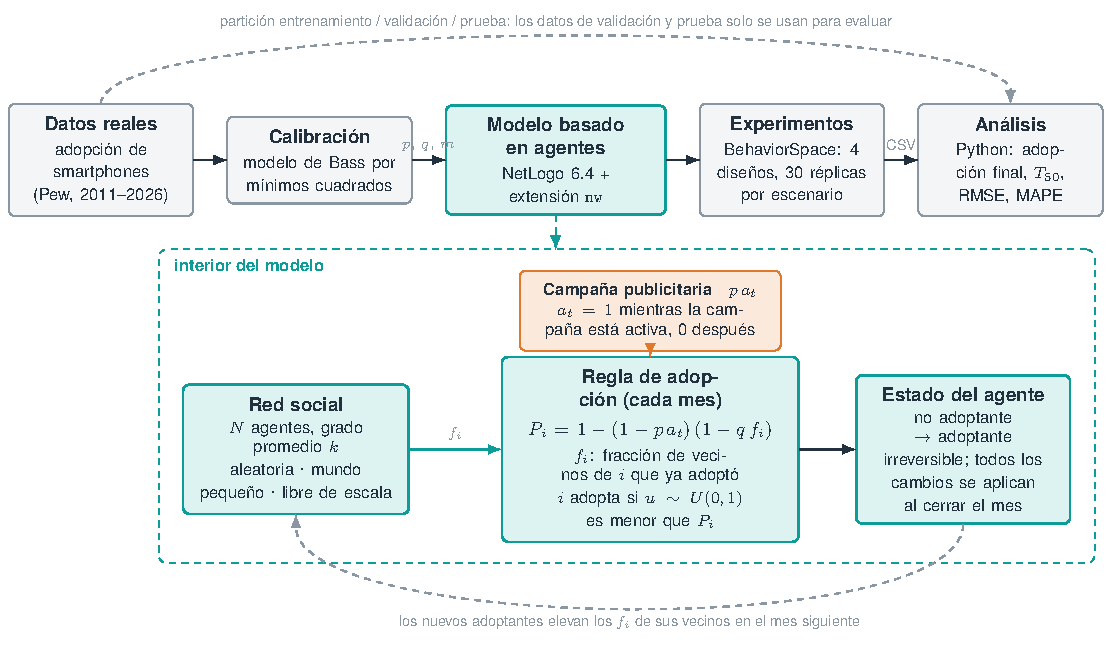
\includegraphics[width=0.88\textwidth]{esquema_sistema.pdf}
  \caption{Esquema del sistema. Arriba, el flujo de trabajo. Abajo, el interior del modelo: la red entrega la fracción de vecinos adoptantes $f_i$, la campaña entrega la señal $a_t$ y la regla decide si el agente cambia de estado.}
  \label{fig:esquema}
\end{figure}

\subsection{Implementación}

El modelo se implementó en NetLogo~\cite{wilensky1999} con la extensión \texttt{nw}, que genera las redes y mide sus propiedades. \texttt{setup} carga los parámetros del caso elegido (PS5, GTA~6 o libre), crea la red, marca el potencial de mercado y siembra los adoptantes iniciales. \texttt{go} ejecuta un mes en dos pasos: en \texttt{decidir}, cada agente que no ha adoptado calcula $f_i$ y sortea su decisión; en \texttt{actualizar} se aplican todas las decisiones, se registran las medidas y se calcula la curva de~\eqref{eq:bass} como referencia.

\subsection{Calibración y analogía}
\label{sec:calibracion}

\textbf{PS5.} Los parámetros de~\eqref{eq:bass} se estimaron por mínimos cuadrados no lineales con la partición de entrenamiento, tomando $t=0$ en el lanzamiento (12 de noviembre de 2020). El potencial $m$ no se puede estimar bien cuando la serie aún está creciendo, así que se trató como hiperparámetro: para cada valor de $m$ entre 0,80 y 1,00 se estimaron $p$ y $q$, y se eligió el $m$ con menor error en validación. El error bajó hasta el tope de la rejilla, de modo que se usó $m=1$ (toda la base de la PS4). Los coeficientes anuales se pasaron a tasas mensuales ($p/12$ y $q/12$).

\textbf{GTA~6.} Como no tiene ventas, se parametrizó por analogía~\cite{thomas1985} con GTA~V, que salió en 2013 para PS3 y Xbox 360 (\cifraGtaBase\ millones de consolas instaladas). GTA~V vendió 11,2 millones de copias el primer día, según el récord que registró Guinness World Records, \cifraGtavSeisSemanas\ millones a las seis semanas y \cifraGtavMeseta\ millones al año~\cite{taketwo2014}, que equivalen al \cifraGtavMesetaPct\,\% de la base. Se fijó $m$ en ese porcentaje, se tomaron los compradores del primer día como adoptantes iniciales, se usó el mismo $q$ de la PS5 y se ajustó $p$. El resultado es $p=\cifraGtaP$ mensual, con un error de \cifraGtaRmse\ puntos. En este caso la publicidad pesa unas \cifraGtaRazonPQ\ veces más que la imitación, al contrario que en la PS5. GTA~6 se modela sobre los dueños de PS5 con $m=\cifraGtaM$\,\%, \cifraGtaIniciales\,\% de compradores el primer día y esos mismos $p$ y $q$.

\section{Conjunto de datos}
\label{sec:datos}

\textbf{Serie real.} La serie principal son las unidades de PS5 vendidas a tiendas que Sony Interactive Entertainment publica cada trimestre fiscal~\cite{sony2026}. Tiene \cifraTrimestres\ trimestres, desde el del lanzamiento (diciembre de 2020) hasta septiembre de 2026, y va de \cifraPsUnidadesIni\ a \cifraPsUnidadesFin\ millones acumulados. El porcentaje de adopción se calcula sobre la base instalada de la generación anterior, la PS4, que según la misma fuente supera los \cifraUniverso\ millones de unidades. Ese universo se fijó antes de mirar la partición de prueba. La Tabla~\ref{tab:datos} muestra algunos ejemplos. La serie de GTA~V tiene cinco valores acumulados entre septiembre de 2013 y agosto de 2014 (\cifraGtavSerie\ millones); el primero es el de Guinness y los demás son de Take-Two.

\begin{table}[htb]
\centering
\caption{Cinco de los 24 trimestres de la serie real: unidades de PS5 vendidas a tiendas (millones), acumulado y porcentaje de la base de PS4 (117 M).}
\label{tab:datos}
\small
\setlength{\tabcolsep}{4pt}
\begin{tabular}{llrrrl}
\toprule
trimestre & cierre & unidades & acumulado & \% base PS4 & partición \\
\midrule
FY2020~Q3 & 31-dic-2020 & 4,5 & 4,5 & 3,8 & entrenamiento \\
FY2022~Q3 & 31-dic-2022 & 7,1 & 32,1 & 27,4 & entrenamiento \\
FY2024~Q3 & 31-dic-2024 & 9,5 & 75,0 & 64,1 & validación \\
FY2025~Q3 & 31-dic-2025 & 7,9 & 92,2 & 78,8 & prueba \\
FY2026~Q2 & 30-sep-2026 & 2,6 & 97,9 & 83,7 & prueba \\
\bottomrule
\end{tabular}
\end{table}


\textbf{Datos simulados.} Cada experimento exporta una fila por corrida y por mes, con los parámetros y las medidas. En total son \cifraCorridas\ corridas de 1000 agentes y \cifraFilas\ filas en archivos CSV.

\section{Diseño experimental}
\label{sec:diseno}

\textbf{Partición.} La serie de la PS5 se dividió en orden cronológico. El entrenamiento va de diciembre de 2020 a diciembre de 2023 (\cifraObsEnt\ trimestres) y sirve para estimar $p$ y $q$. La validación va de marzo a diciembre de 2024 (\cifraObsVal\ trimestres) y sirve para elegir $m$ y la estructura de la red. La prueba va de marzo de 2025 a septiembre de 2026 (\cifraObsPru\ trimestres) y no interviene en ninguna decisión. Como control adicional se usa un dato de Sony posterior a la serie: más de 100 millones de unidades al 10 de noviembre de 2026 (\cifraControlReal\,\% de la base).

\textbf{Medidas de desempeño.} La principal es el \emph{porcentaje de adopción al final del período}: la fracción de la población que ha adoptado a los \cifraHorizontePs\ meses del lanzamiento en la PS5 y a los \cifraHorizonteGta\ meses en GTA~6. También se reportan el mes en que se alcanza el 50\,\% y el mes con más adoptantes nuevos. Para comparar con la serie real se usan, en cada partición, la raíz del error cuadrático medio (RMSE, en puntos porcentuales) y el error porcentual absoluto medio (MAPE) entre la curva simulada promedio y el valor observado al cierre de cada trimestre. Cada escenario se repite 30 veces y se reportan la media y el intervalo de confianza del 95\,\% ($t$ de Student). El intervalo recoge la variación entre réplicas, no la incertidumbre de $p$, $q$ y $m$.

\textbf{Escenarios.} La Tabla~\ref{tab:experimentos} resume los cuatro experimentos. E1, E2 y E3 se corren para los dos casos con $N=1000$ agentes y la red de mundo pequeño con $k=16$, que fue la elegida en validación, salvo en el factor que cambia. En la PS5 se siembra un 2,5\,\% de adoptantes iniciales (los innovadores de Rogers~\cite{rogers2003}) para que el escenario sin campaña pueda arrancar; en GTA~6 se siembran los compradores del primer día. En los escenarios sin campaña, $p=0$ desde el lanzamiento. Esto elimina toda la influencia externa, así que la diferencia con el escenario con campaña es una cota superior del efecto de la publicidad.

\begin{table}[htb]
  \centering
  \caption{Experimentos (30 réplicas por combinación). E1, E2 y E3 se corren para PS5 y GTA~6.}
  \label{tab:experimentos}
  \footnotesize
  \setlength{\tabcolsep}{4pt}
  \begin{tabular}{llr}
    \toprule
    exp. & factores y niveles & corridas \\
    \midrule
    E1 & publicidad \{sin, con\} $\times$ densidad $k\in\{2,4,6,8,12,16\}$ & 720 \\
    E2 & publicidad $\times$ topología \{aleatoria, mundo pequeño, libre de escala\} & 360 \\
    E3 & duración de la campaña \{0, 1, 3, 6, 12, 24 meses, permanente\} & 420 \\
    E4 & calibración (PS5): topología (3) $\times$ $k\in\{4,8,16\}$, 74 meses & 270 \\
    \bottomrule
  \end{tabular}
\end{table}

\textbf{Verificación.} La regla se programó por segunda vez en Python con \texttt{networkx} y se repitieron los cuatro experimentos. En los \cifraVerifEscenarios\ escenarios, la adopción final media de las dos implementaciones difiere en \cifraVerifDifMedia\ puntos en promedio y en \cifraVerifDifMax\ puntos como máximo. Con la prueba $t$ de Welch y la corrección de Holm, \cifraVerifHolm. Además, con una red completa la regla reproduce la curva de Bass (diferencia máxima de \cifraVerifBassMax\ puntos).

\section{Resultados}
\label{sec:resultados}

\subsection{Calibración y validación con la PS5}

El ajuste en entrenamiento dio $p=\cifraBassP$ y $q=\cifraBassQ$ anuales, con $m=\cifraBassM$\,\%. La imitación pesa \cifraBassRazonQP\ veces más que la publicidad, lo que explica la forma de S de la serie. Con esos mismos coeficientes, el modelo de agentes difunde más despacio que el modelo agregado, porque parte de la influencia de cada adoptante recae en vecinos que ya adoptaron. Por eso las nueve redes probadas quedan por debajo de la serie real, y el error disminuye cuando aumenta $k$ (Tabla~\ref{tab:calibracion}).

En validación se eligió la \cifraAbmSelRedNombre\ con $k=\cifraAbmSelK$, con un error de \cifraAbmRmseVal\ puntos. La \cifraAbmSegundaRedNombre\ con $k=\cifraAbmSegundaK$ quedó muy cerca (\cifraAbmSegundaRmseVal\ puntos), así que la diferencia entre las dos no es concluyente. En la partición de prueba el modelo de agentes tiene un error de \cifraAbmRmsePru\ puntos (MAPE de \cifraAbmMapePru\,\%), mayor que el del modelo agregado (\cifraBassRmsePru\ puntos). Los dos modelos quedan también por debajo del dato de control de noviembre de 2026: \cifraControlAbm\,\% y \cifraControlBass\,\%, frente a más de \cifraControlReal\,\% (Figura~\ref{fig:calibracion}). Esto indica que $m=1$ se queda corto: un ajuste con toda la serie sugiere que la PS5 llegará a unos \cifraBassMLibreM\ millones.

\begin{table}[htb]
\centering
\caption{RMSE (puntos) del modelo de agentes en validación / prueba, por topología y $k$; $\star$: elegida en validación. Bass: 2,14 / 3,22.}
\label{tab:calibracion}
\small
\setlength{\tabcolsep}{4pt}
\begin{tabular}{lrrr}
\toprule
red & $k=4$ & $k=8$ & $k=16$ \\
\midrule
aleatoria & 7,06 / 9,92 & 4,15 / 5,84 & 3,31 / 4,55 \\
mundo pequeño & 6,22 / 8,91 & 3,94 / 6,07 & 3,20 / 4,91$^\star$ \\
libre de escala & 6,82 / 9,38 & 4,09 / 6,07 & 3,86 / 5,10 \\
\bottomrule
\end{tabular}
\end{table}


\begin{figure}[htb]
  \centering
  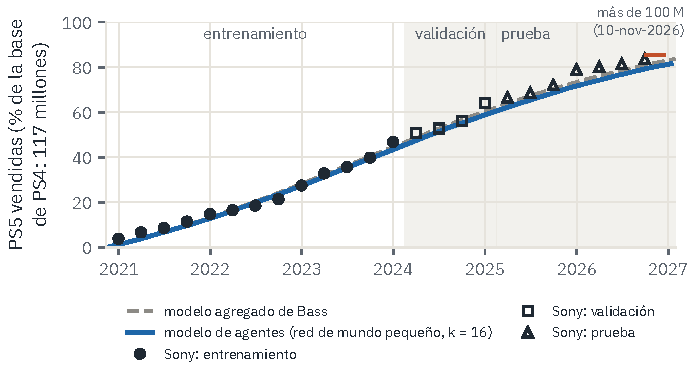
\includegraphics[width=0.72\textwidth]{fig_calibracion.pdf}
  \caption{Serie de la PS5 por partición, curva de Bass ajustada y curva media del modelo de agentes con la red elegida en validación (banda: IC 95\,\%). El trazo horizontal marca el dato de control de Sony del 10 de noviembre de 2026.}
  \label{fig:calibracion}
\end{figure}

\subsection{Publicidad y densidad de la red}

La Figura~\ref{fig:escenarios}(a, b) muestra las curvas de E1 para la red más dispersa y la más densa. En la PS5, sin publicidad la adopción a seis años va del \cifraPsSinKDos\,\% con $k=2$ al \cifraPsSinKDieciseis\,\% con $k=16$, y nunca alcanza el 50\,\%. Con campaña la curva toma forma de S, cruza el 50\,\% hacia el mes \cifraTcincuentaPsConKDieciseis\ con $k=16$ y termina entre el \cifraPsConMin\,\% y el \cifraPsConMax\,\%.

La densidad importa más cuando no hay publicidad. Sin campaña, pasar de $k=2$ a $k=16$ multiplica la adopción por \cifraPsSinRazon\ (\cifraPsSinGanancia\ puntos más), porque con más contactos la influencia sale antes de los grupos locales. Con campaña, el mismo cambio solo la multiplica por \cifraPsConRazon\ (\cifraPsConGanancia\ puntos más), porque la publicidad ya reparte adoptantes por toda la red.

En GTA~6 la campaña decide el resultado. Con ella se alcanza el potencial (entre \cifraGtaConMin\,\% y \cifraGtaConMax\,\%) y el mes con más compras es el \cifraMesPicoGtaConKDieciseis. Sin ella, la adopción apenas supera a los compradores del primer día (\cifraGtaSinMin\,\% a \cifraGtaSinMax\,\%), sin importar la densidad.

\begin{figure}[htb]
  \centering
  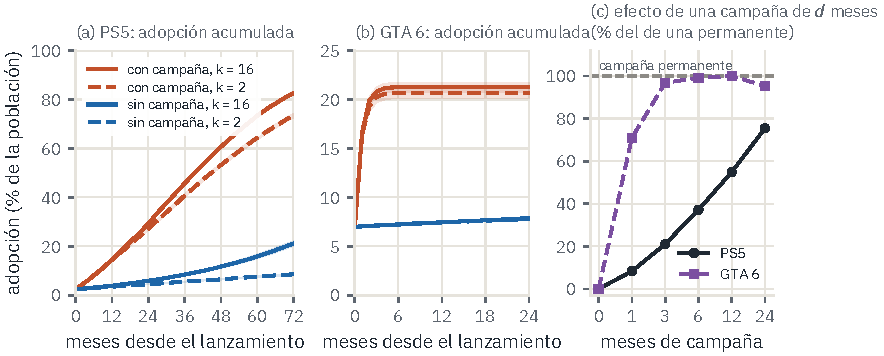
\includegraphics[width=\textwidth]{fig_escenarios.pdf}
  \caption{(a, b) Curvas medias de adopción con y sin campaña en redes de mundo pequeño con $k=2$ y $k=16$, para la PS5 (a) y GTA~6 (b); la banda es el IC 95\,\%. (c) Efecto de una campaña de $d$ meses como porcentaje del efecto de una campaña permanente, $(A_d-A_0)/(A_{\text{perm}}-A_0)$. Los valores por encima de 100\,\% se deben a la variación entre réplicas.}
  \label{fig:escenarios}
\end{figure}

\subsection{Topología de la red}

En E2 las tres topologías tienen $k=16$, pero la de mundo pequeño tiene mucho más agrupamiento: $C=\cifraEstMundoC$, frente a \cifraEstAleatoriaC\ en la aleatoria y \cifraEstEscalaC\ en la libre de escala. Con campaña, las tres dan casi el mismo resultado en la PS5 (\cifraTopoPsConMin\,\% a \cifraTopoPsConMax\,\%). Sin campaña, la de mundo pequeño es la más lenta: \cifraTopoPsSinMundo\,\%, frente a \cifraTopoPsSinAleatoria\,\% en la aleatoria y \cifraTopoPsSinEscala\,\% en la libre de escala. La razón es que la influencia se queda dentro de grupos que ya adoptaron. La libre de escala es la más variable (desviación estándar de \cifraTopoPsSinEscalaDe\ puntos, frente a \cifraTopoPsSinAleatoriaDe\ y \cifraTopoPsSinMundoDe), porque su resultado depende de que un nodo muy conectado adopte pronto. En GTA~6 la topología no cambia el resultado.

\subsection{Duración de la campaña}

En E3 la campaña se interrumpe después de cierto número de meses (Figura~\ref{fig:escenarios}(c)). En GTA~6, un mes de campaña consigue el \cifraFraccionGtaDUno\,\% del efecto de una campaña permanente y tres meses el \cifraFraccionGtaDTres\,\%: casi todo se decide en el lanzamiento. En la PS5 el efecto se acumula poco a poco. Un año de campaña consigue el \cifraFraccionPsDDoce\,\% del efecto y dos años el \cifraFraccionPsDVeinticuatro\,\% (\cifraDurPsDVeinticuatro\,\% de adopción, frente a \cifraDurPsDPermanente\,\% con campaña permanente), porque la imitación necesita tiempo para sostener la difusión.

\section{Conclusiones}
\label{sec:conclusiones}

El modelo reproduce la partición de prueba de la PS5 con un error de \cifraAbmRmsePru\ puntos y deja tres conclusiones. Primera: en una tecnología que se difunde por imitación, como la PS5, la publicidad es necesaria para que la difusión despegue (como máximo \cifraPsSinMaxGlobal\,\% de adopción sin campaña, frente a \cifraPsConMin\,\% o más con ella) y su efecto se acumula con los meses. Segunda: en un lanzamiento dominado por la publicidad, como GTA~6, el primer mes de campaña decide el resultado y la red casi no influye. Tercera: la densidad y la topología de la red importan sobre todo cuando no hay publicidad.

El trabajo tiene varias limitaciones. Todos los agentes comparten los mismos coeficientes y la red no cambia. Las unidades vendidas a tiendas no son exactamente compradores. Los parámetros de GTA~6 son hipotéticos; si se duplican su potencial y sus compradores del primer día, cambia el nivel de adopción (\cifraSensDobleSin\,\% sin campaña y \cifraSensDobleCon\,\% con ella), pero no el papel de la campaña. Queda comparar el escenario de GTA~6 con sus primeras ventas.

\bibliographystyle{splncs04}
\bibliography{referencias}

\end{document}
